\chapter{\ifproject%
\ifenglish Project Structure and Methodology\else โครงสร้างและขั้นตอนการทำงาน\fi
\else%
\ifenglish Project Structure\else โครงสร้างของโครงงาน\fi
\fi
}

ในบทนี ้ จะกล่าวถึงหลักการ,  การนําทฤษฎีที่เกี่ยวข้องมาประยุกต์ใช้  และการออกแบบของระบบ


\makeatletter

% \renewcommand\section{\@startsection {section}{1}{\z@}%
%                                    {13.5ex \@plus -1ex \@minus -.2ex}%
%                                    {2.3ex \@plus.2ex}%
%                                    {\normalfont\large\bfseries}}

\makeatother
%\vspace{2ex}
% \titleformat{\section}{\normalfont\bfseries}{\thesection}{1em}{}
% \titlespacing*{\section}{0pt}{10ex}{0pt}
\section{โครงสร้างของระบบ}
% \ref{fig:Overall project structure}
\begin{figure}[h]
  \begin{center}
  % 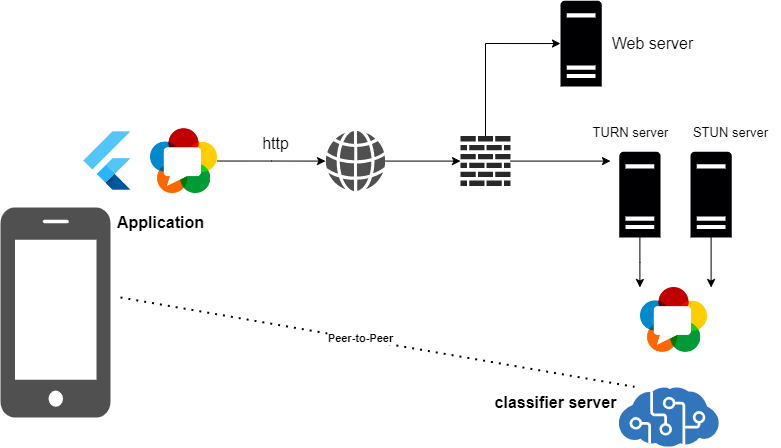
\includegraphics{pic/webrtc.png}
  \vspace{0.5cm}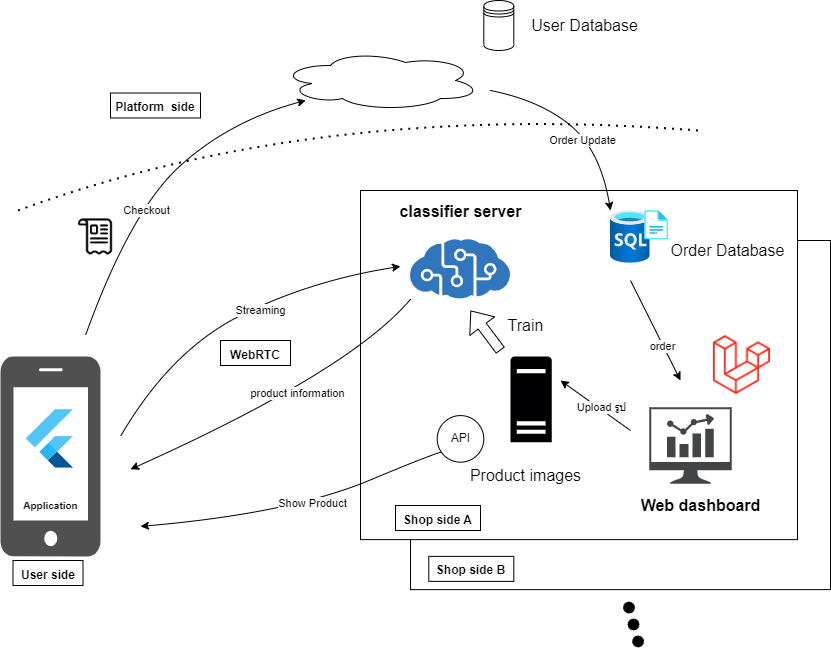
\includegraphics[scale=0.5]{pic/overall_2.png}
  \end{center}
  
  \caption[Overall project structure]{Overall project structure}
  \label{fig:Overall project structure}
  \end{figure}
\section{เตรียมชุดข้อมูลฝึกสอน}
ข้อมูลที่ใช้ในการ train mode โดยมีสินค้าประมาณ 100 ชนิด โดยจัดเก็บข้อมูลใช้กล้องมือถือ ในการถ่ายภาพในมุมต่างๆ
ของสินค้าชนิดนั้นๆ ตามมุมต่างๆ จำนวนชนิดละ N รูป โดยจัดเก็บใน  และทำการดึงข้อมูลมา train ผ่าน Google Colab
 โดยโครงสร้างการเก็บข้อมูลจะเป็นดังรูป

\begin{center}
  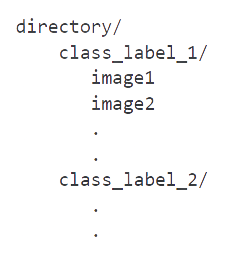
\includegraphics[scale=0.35]{pic/st.png}
\end{center}

\section{การเพิ่ม traing data}
โดยสินค้า 1 ชนิด ทำการถ่ายภาพ 6 รูป ในมุมที่แตกต่างกัน 
โดยในแต่ละ 1 รูปภาพที่ถ่าย จะแปลงเป็นรูปภาพ RGB ขนาด 224x224 pixel
และในแต่ละรูปเพื่อให้มี train dataset จำนวนมาก นำไปหมุนและกลับด้าน ด้วยมุม -20,-15,-10,-5,0,5,10,15,20 องศา
โดย 1 รูปภาพผ่านการ generate datasets จะกลายเป็น 18 รูปภาพซึ่งมีความแตกต่างกันเล็กน้อย
\begin{figure}[h]
  \begin{center}
  % 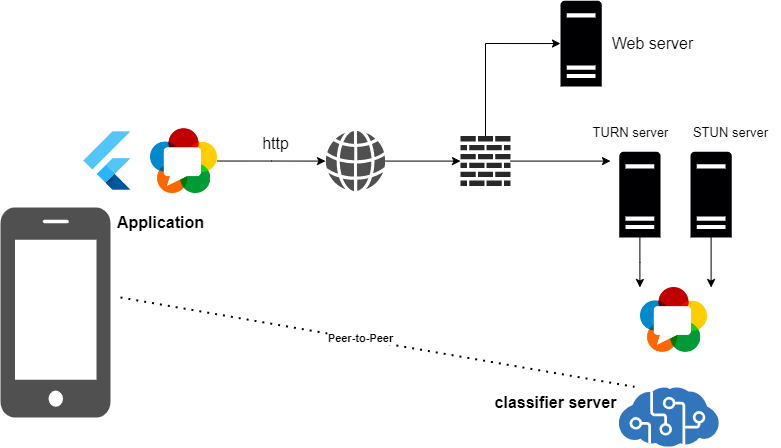
\includegraphics{pic/webrtc.png}
  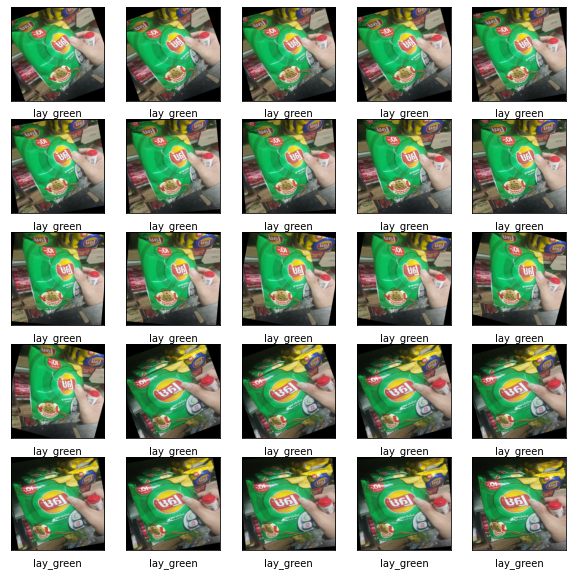
\includegraphics[scale=0.4]{pic/genmore.png}
  \end{center}
  
  \caption[Dataset generator]{Dataset generator}
  \label{fig:Dataset generator}
  \end{figure}

  \newpage
\subsection{Model Architecture}
โดยโมเดลในโครงงานนี้จะใช้ Xception pre-trained มาใช้ในการแยกคุณลักษณะเด่นของรูปภาพ  และสร้างโมเดลมาต่อท้ายเพื่อ 
เรียนรู้ลักษณะเด่นจากที่ Xception ทำการแยกออกมาได้
\begin{center}
  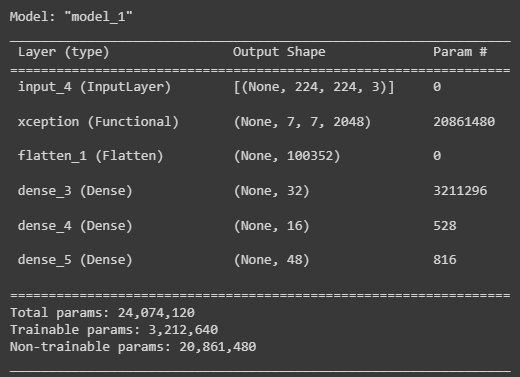
\includegraphics[scale=0.45]{pic/model.png}
\end{center}
  
โดยต่อท้ายด้วย fully connected node ที่เรียกว่า Dense layer ซึ่งทำหน้าที่เป็น classifier 
 โดยมี output layer ที่มีจำนวน node เท่ากับจำนวนสินค้า สำหรับการ classify ชนิดของ
  products จาก รูปภาพ
 
% \section{Product database}
% Section 2 text.

 

 
% \subsection{Transfer Learning}

Subsection 1 text

\section{classification products}
จากรูปภาพใน 48 class ผ่านการ generate datasets จะมี dataset ทั้งหมด 4432 sample
 ทำการแบ่งเป็น train 3546 sample และ  886 sample สำหรับการ evaluate 
โดยจาก train 3546 แบ่ง 50\% สำหรับการ validation ในระหว่างการ train model

\par ผลลัพธ์ จากการ train \& validation ด้วย 3546 sample เป็นจำนวน 40 Epoch
\begin{figure}[h]
  \begin{center}
  % 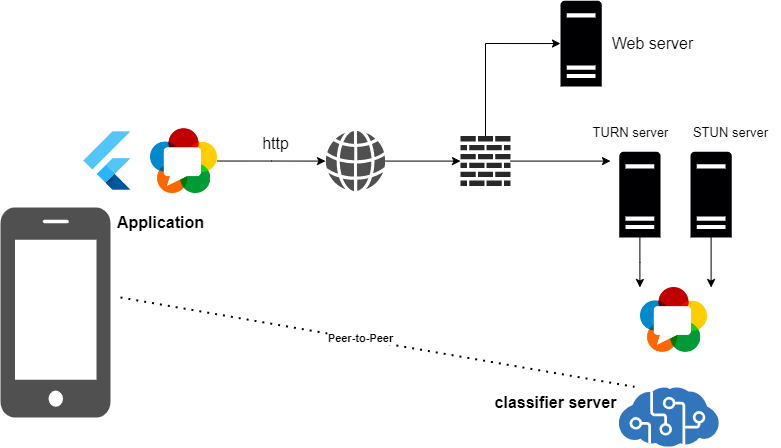
\includegraphics{pic/webrtc.png}
  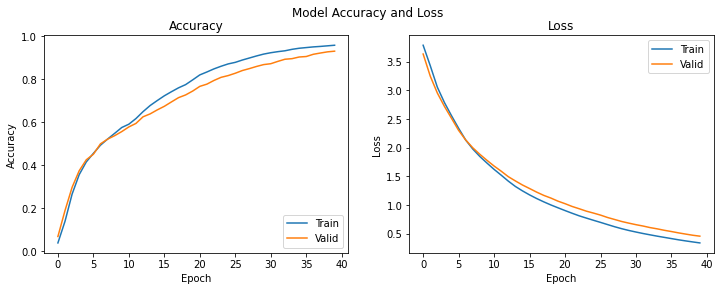
\includegraphics[scale=0.45]{pic/train.png}
  \end{center}
  
  \caption[Train results]{Train results}
  \label{fig:Train results}
  \end{figure}

  % โดยเมื่อนำ evaluate มาหา cross_entropy 0.23343226313591003, 0.944695234298706 accuracy

  และทำการ save model ที่มีความแม่นยำระดับนึง
   สำหรับเป็น service ในการ classify products ของ application ผ่าน aiortc  และเว็บ WebRTC

  % score (cross_entropy, accuracy):
%  [0.23343226313591003, 0.944695234298706]

% \begin{figure}[h]
% \begin{center}
% % 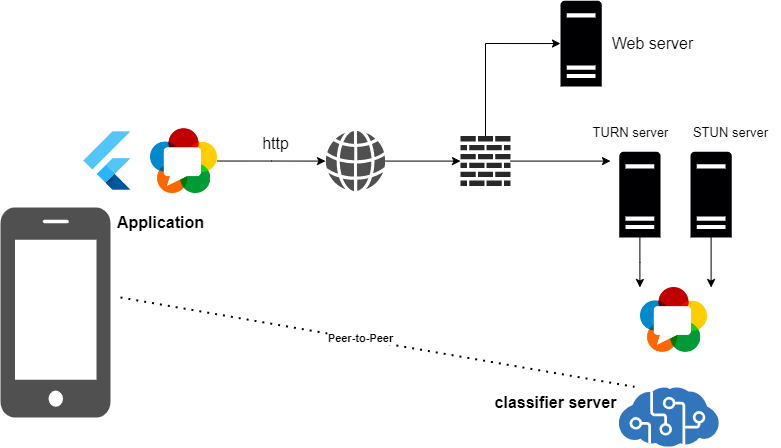
\includegraphics{pic/webrtc.png}
% 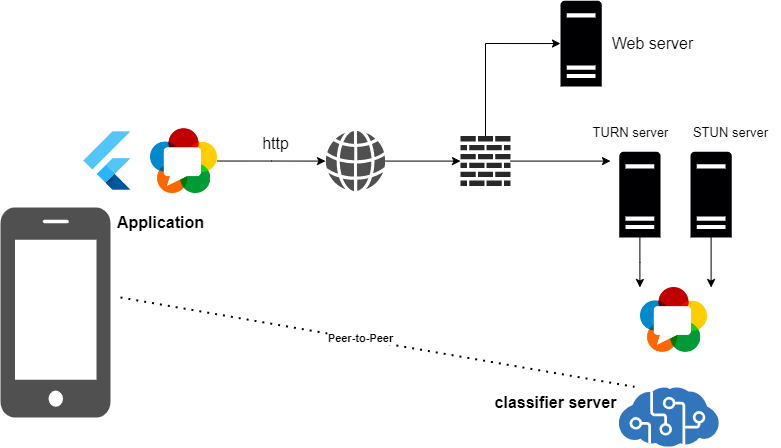
\includegraphics[scale=0.5]{pic/webrtc.png}
% \end{center}

% \caption[webrtc structure]{webrtc structure}
% \label{fig:webrtc structure}
% \end{figure}
\newpage

\section{การพัฒนา Mobile Application}
ใช้ Flutter ในการสร้าง Mobile Application ในส่วนของผู้ใช้โดยใช้ service ของ WebRTC ติดต่อกับ Classification server ที่ได้ทำการฝึกสอนไว้แล้ว
โดยจะแอพลิเคชันจะมีฟังก์ชันที่ทำการสตรีมมิ่งภาพสินค้าที่ลูกค้าถ่ายผ่าน WebRTC ไปยัง server ของทางร้านซึ่งมี Model classifier อยู่
จากนั้น Server ของทางร้านจะ Classifiy ว่าเป็นสินค้าชนิดใด และตอบกลับมายังแอพลิเคชันเพื่อแสดงผลให้กับผู้ใช้งาน
\subsection{Requirement Specification}  

\begin{enumerate}
  \item ผู้คนทั่วไปสามารถลงทะเบียนเข้าใช้งานได้ผ่าน SSO อีเมล์ และหมายเลขโทรศัพท์มือถือ
  \item สามารถเชื่อมต่อกับข้อมูลร้านค้าได้ผ่านการแสกนคิวอาร์โค้ดเข้าใช้งานร้านค้า
  \item สามารถใช้กล้องโทรศัพท์มือถือแสกนสินค้าเพื่อสตรีมภาพ Classification server เพื่อทำการดึงข้อมูลสินค้าจาก Server ของร้านค้ามาแสดงผลบนแอพลิเคชัน
  \item สามารถเพิ่มหรือลดสินค้าในตะกร้าได้
  \item สามารถทำการชำระเงินได้ผ่าน Payment gateway ในตัวแอพลิเคชัน
  \item สามารถ Checkout จากร้านค้าผ่านการแสกนคิวอาร์โค้ดออกจากร้านค้า
 
\end{enumerate}


\section{การเตรียมฐานข้อมูล}
ในการเก็บฐานข้อมูลจะแบ่งเป็นฐานข้อมูลสองตัว โดยใช้ Supabase 
ในการสร้างโครงการ และจัดฐานข้อมูลทั้งหมดแบบ SQL ได้แก่ 
\subsection{ฐานข้อมูลของระบบ}
สำหรับเก็บข้อมูลร้านค้าที่เข้าร่วม และประวัติการซื้อสินค้าของผู้ใช้งานแอพลิเคชันมือถือ ซึ่งมี Database schema ดังนี้ 
\begin{figure}[h]
\begin{center}
  % 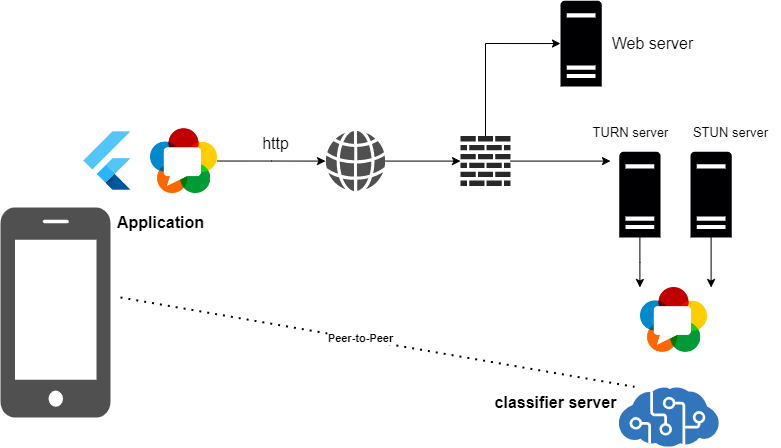
\includegraphics{pic/webrtc.png}
  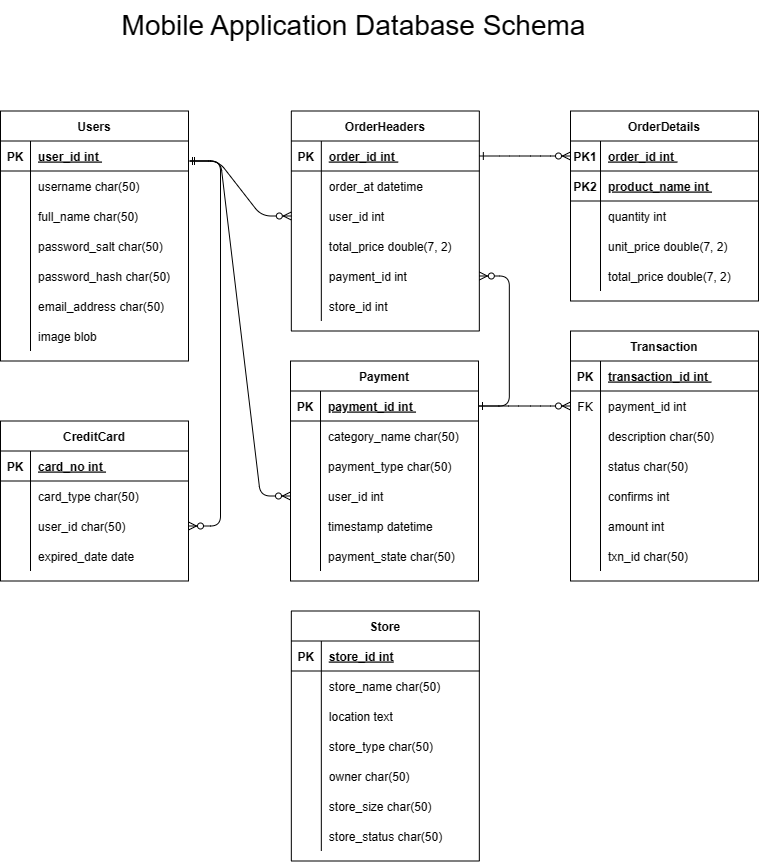
\includegraphics[scale=0.3]{pic/datamobile.png}
  \end{center}
  
  \caption[Mobile Application Database Schema]{Mobile Application Database Schema}
  \label{fig:Mobile Application Database Schema}
  \end{figure}


  
\subsection{ฐานข้อมูลในแต่ละร้านค้า}
สำหรับเก็บข้อมูลสินค้า และประวัติยอดขายของร้านค้า โดยร้านค้าแต่ละร้านจะมีฐานข้อมูลเป็นของตนเองเพื่อใช้งานกับ Server ของร้านนั้น ๆ
 โดยตรง ซึ่งจะมี Database schema ดังนี้ 

 \begin{figure}[h]
  \begin{center}
    % 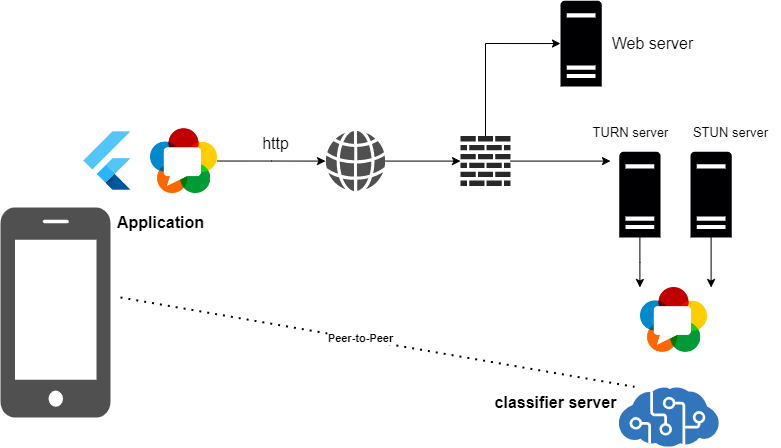
\includegraphics{pic/webrtc.png}
    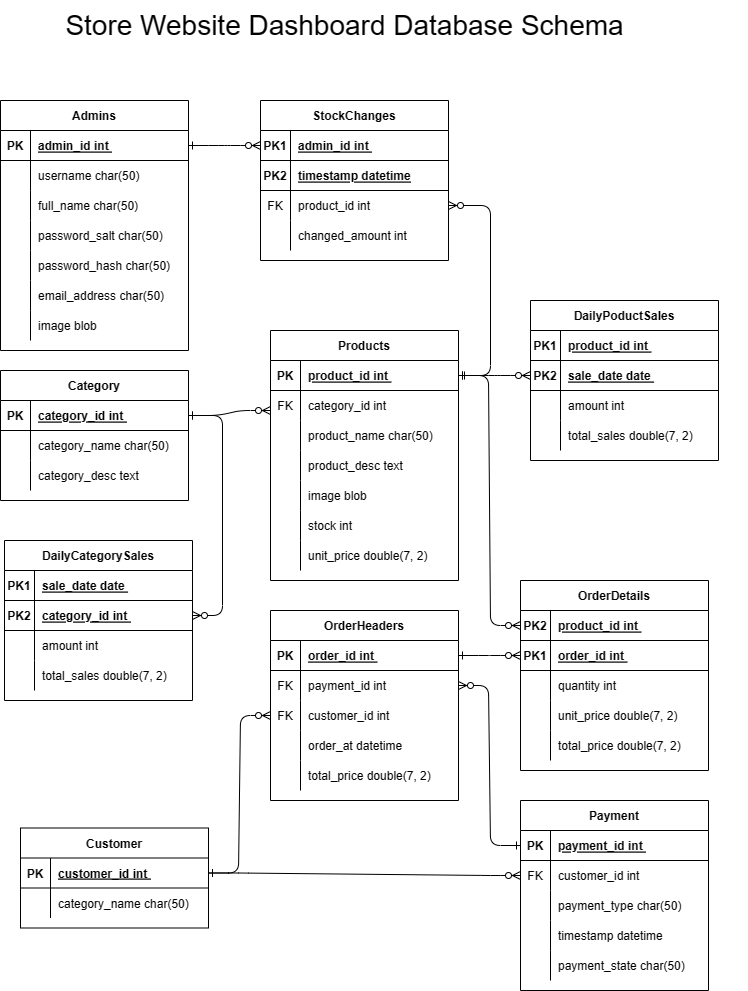
\includegraphics[scale=0.3]{pic/dataweb.png}
    \end{center}
    
    \caption[Store Website Dashboard Database Schema]{Store Website Dashboard Database Schema}
    \label{fig:Store Website Dashboard Database Schema}
    \end{figure}
  
\section{การพัฒนา Website Dashboard }


ออกแบบ UI/UX ของ Wedsite Dashboard และ Mobile Application ด้วย Figma
หลังจากการออกแบบ และจัดการตั้งค่าฐานข้อมูลเสร็จแล้ว
 ก็จะพัฒนาในส่วนของเว็บไซต์ทางฝั่งร้านค้าโดยใช้ Supabase ในการโฮสติ้งเว็บไซต์ 
 และเชื่อมต่อกับฐานข้อมูลที่ได้ตั้งค่าไว้ โดยใช้ Flask framework 
 ในการจัดการ API และ Python ในการจัดการระบบ Backend ของเว็บไซต์โดยใช้ SQLAlchemy
  ในการดึงข้อมูลจากฐานข้อมูล Requirement Specification ดังนี้

  \begin{enumerate}
    \item สามารถเข้าใช้งานได้ผ่านการยืนยันตัวตนเป็น Administers เท่านั้น โดยสามารถมีได้ 1-5 คน
    \item สามารถดูคลังสินค้า และแก้ไขข้อมูลสินค้าในแต่ละชนิดได้แบบเรียลไทม์
    \item สามารถดูสถิติยอดขายสินค้าได้ทั้งแบบรายวัน รายเดือน และรายปี โดยแบ่งได้ 2 แบบ คือตามชนิดสินค้า และประเภทสินค้า
    \item สามารถดูประวัติการขายตามออเดอร์ของลูกค้าแต่ละคนได้ และดูข้อมูลของแต่ละออร์เดอร์ได้
\end{enumerate}



 

\section{การทดสอบการทำงานของซอร์ฟแวร์}
การทดสอบการทำงานของระบบ สามารถแบ่งเป็นขั้นตอนดังนี้
\subsection{Unit testing}
การทดสอบความถูกต้องของการทำงานในแต่ละฟังก์ชันหลักของระบบแยกกัน โดยยังไม่รวมแต่ละ Component เข้าด้วยกัน ซึ่งได้แก่
\begin{enumerate}
  \item Classification system
  \item Website dashboard
  \item Mobile Application
\end{enumerate}

\subsection{Integration testing}
การทดสอบการทำงานเมื่อรวมระบบย่อยทั้งหมดเข้าด้วยกัน โดยหลัก ๆ
 จะทดสอบในเรื่อง API ว่ามีการรับส่งข้อมูลดุถูกต้องหรือไม่ และทำงานโดยรวมได้ถูกต้องทั้งหมดหรือไม่
\subsection{System testing}
การทดสอบระบบซึ่งแต่ละโมดูลข้างต้นจะถูกรวม และทดสอบเป็นกลุ่ม 
เพื่อประเมินความสอดคล้องของระบบว่าทำงานได้ตามที่กำหนดไว้หรือไม่
\subsection{Acceptance testing}
การทดสอบระบบโดยดูภาพรวมของการทำงาน ว่ามีการตอบสนองความต้องการของผู้ใช้ทั้งในส่วนของฟังก์ชันการทำงาน 
และประสิทธิภาพการทำงาน ว่าสอดคล้องกับลักษณะของความต้องการของซอฟต์แวร์หรือไม่ 
โดยใช้การทดสอบแบบ Functional testing (Black box testing)
\section{แผนภาพกระแสข้อมูล (Data Flow Diagram)}
\begin{figure}[h]
  \begin{center}
  % 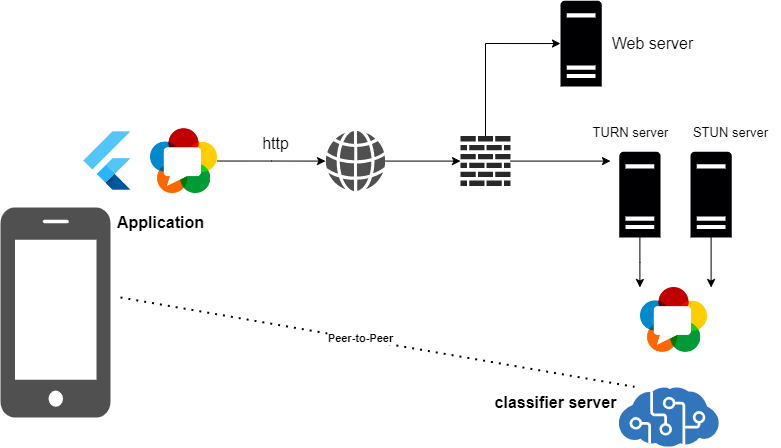
\includegraphics{pic/webrtc.png}
  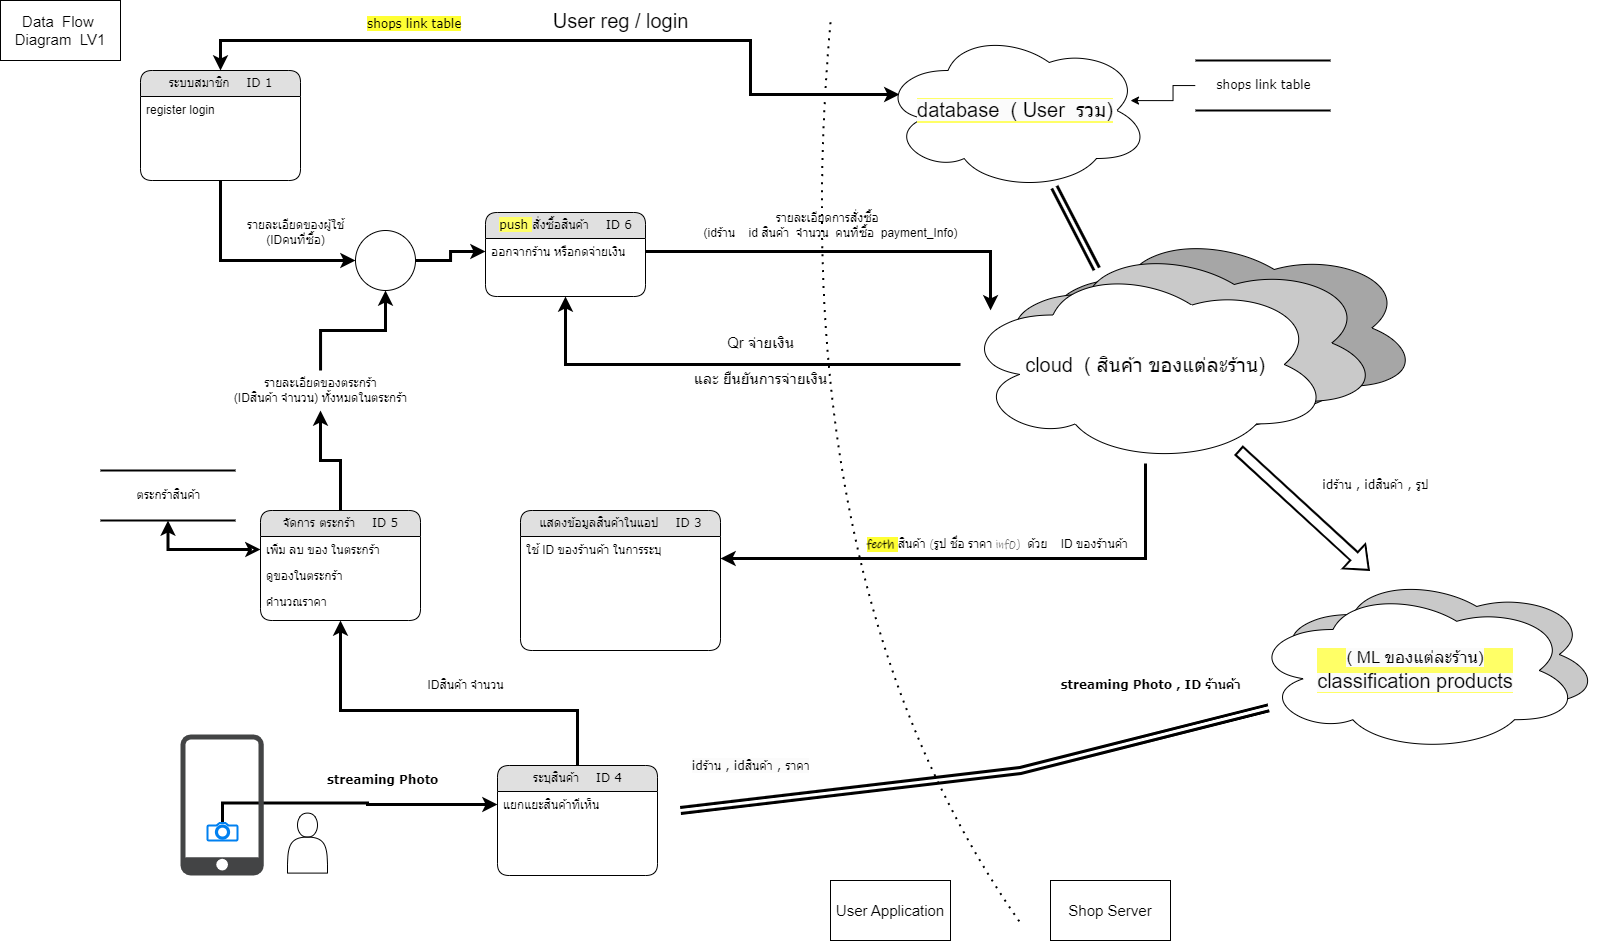
\includegraphics[scale=0.25]{pic/dataflow-lv0.png}
  \end{center}
  
  \caption[Data Flow Diagram]{Data Flow Diagram}
  \label{fig:Data Flow Diagram}
  \end{figure}
  

% \subsection{The Black Kitten}
  % One thing was certain, that the WHITE kitten had had nothing to
% do with it:---it was the black kitten's fault entirely



% ~\cite{aiw}. 




%  For the
% white kitten had been having its face washed by the old cat for
% the last quarter of an hour (and bearing it pretty well,
% considering); so you see that it COULDN'T have had any hand in
% the mischief.

%   The way Dinah washed her children's faces was this:  first she
% held the poor thing down by its ear with one paw, and then with
% the other paw she rubbed its face all over, the wrong way,
% beginning at the nose:  and just now, as I said, she was hard at
% work on the white kitten, which was lying quite still and trying
% to purr---no doubt feeling that it was all meant for its good.

%   But the black kitten had been finished with earlier in the
% afternoon, and so, while Alice was sitting curled up in a corner
% of the great arm-chair, half talking to herself and half asleep,
% the kitten had been having a grand game of romps with the ball of
% worsted Alice had been trying to wind up, and had been rolling it
% up and down till it had all come undone again; and there it was,
% spread over the hearth-rug, all knots and tangles, with the
% kitten running after its own tail in the middle.

% \subsection{The Reproach}

  